% Risultati della versione precedente (modello v1, riferimento legacy max-abs su REMESH e insiemi collegati).
% Estratti da main_cvpr_draft.tex il 12 ottobre 2026 (righe 236-335, 363-437, 555-642, 714-908, 1046-1748),
% testo e numeri invariati salvo: titoli abbassati di un livello, riferimenti al main con prefisso M-, figure con
% render di mesh BFM tolte (licenza BFM: niente derivati), sezione dei costi spostata in sec:cost. Le fonti dei
% numeri sono quelle della bozza (versione NeurIPS, main_short.tex, e i commenti della bozza).

\subsection{Model and training objective (v1; the loss terms are shared by the factorized head)}
\label{sec:legacy_objective}
\subsubsection{Mesh-Agnostic Encoder}
\label{sec:encoder}
We learn a shared embedding space for heterogeneous 3D face meshes. By mesh-agnostic, we mean that the encoder does not require a fixed vertex count, mesh connectivity, or template correspondence across inputs. Given an input mesh $M$, an encoder $f_\theta$ maps it to a latent vector $z=f_\theta(M)\in\mathbb{R}^d$. The learned dissimilarity between two meshes is defined as Euclidean distance in latent space:
\begin{equation}
D_{\theta}(M_i,M_j)
=
\left\|
f_{\theta}(M_i)-f_{\theta}(M_j)
\right\|_2 .
\end{equation}
Unlike registration-based geometric pipelines, this distance does not require pairwise alignment, ICP, non-rigid registration, landmarks, or dense correspondence at inference time.

We use an encoder-only surface network based on DiffusionNet~\cite{diffusionet}. 
For each triangular mesh $M=(V,F)$, vertices are centered and normalized, and the network receives normalized XYZ coordinates together with precomputed geometric operators, including mass, Laplacian, eigensystem, and gradient operators. These operators provide a geometry-aware bias that helps generalization across mesh connectivity and sampling changes. Because the encoder consumes raw XYZ coordinates, it is not invariant to rigid motions (rotation and translation) by construction; robustness to such transformations is only encouraged, not guaranteed, through online rigid-motion augmentation during training (random per-axis rotations up to $12^\circ$ and translations with per-axis standard deviation up to $0.03$ in normalized mesh units, applied with probability $0.6$; App.~\ref{app:training_details}), together with cross-topology supervision.

The reported model uses four DiffusionNet blocks with hidden width 128 and outputs a 256-dimensional latent embedding. Vertex features are aggregated by concatenated mean and max pooling followed by a linear projection. The same encoder is shared across all topology variants.
\subsubsection{Training Objective}
\label{sec:training_objective}

Training uses topology-consistent synthetic identities with an exact subject-level
ground-truth distance matrix $D_{\mathrm{GT}}$. Each mini-batch contains multiple
subjects and multiple mesh realizations per subject. Let
$z_{s,m}=f_\theta(x_{s,m})$ be the embedding of realization $m$ of subject $s$,
and define the batch subject embedding as
$\bar z_s = M_s^{-1}\sum_{m=1}^{M_s} z_{s,m}$.

The model is trained with a mixed subject- and mesh-level objective:
\begin{equation}
\begin{split}
\mathcal L ={}&
\lambda_{\mathrm{subj}}
\left(
\mathcal L^{\mathrm{subj}}_{\mathrm{stress}}
+
\lambda_r \mathcal L^{\mathrm{subj}}_{\mathrm{rank}}
\right)
\\
&+
\lambda_{\mathrm{mesh}}
\left(
\mathcal L^{\mathrm{mesh}}_{\mathrm{stress}}
+
\lambda_r \mathcal L^{\mathrm{mesh}}_{\mathrm{rank}}
\right)
+
\lambda_i \mathcal L_{\mathrm{id}} .
\end{split}
\end{equation}
Subject-level terms preserve the identity manifold defined by $D_{\mathrm{GT}}$,
while mesh-level terms expose the model to topology-induced variation. We use
$\lambda_{\mathrm{subj}}=\lambda_{\mathrm{mesh}}=1$, $\lambda_r=0.5$, and
$\lambda_i=0.25$.

\paragraph{Stress and ranking preservation.}
For embeddings $Z$ and valid pairs $\Omega$, latent and ground-truth distances
are matched with a scale-normalized Smooth L1 stress:
\begin{equation}
\mathcal L_{\mathrm{stress}}
=
\frac{1}{|\Omega|}
\sum_{(i,j)\in\Omega}
\operatorname{SmoothL1}
\left(
\frac{\lVert z_i-z_j\rVert_2}{\mu_z+\epsilon},
\frac{D_{\mathrm{GT},ij}}{\mu_{\mathrm{GT}}+\epsilon}
\right),
\end{equation}
where $\mu_z$ and $\mu_{\mathrm{GT}}$ are mean distances over $\Omega$. We apply
this loss at both subject and mesh level. We additionally enforce the ordering
induced by $D_{\mathrm{GT}}$ using a margin-based ranking loss. For subject
triplets $(i,j,k)$ satisfying
$D_{\mathrm{GT}}(i,j)>D_{\mathrm{GT}}(i,k)+\tau$,
\begin{equation}
\mathcal L^{\mathrm{subj}}_{\mathrm{rank}}
=
\mathbb E
\left[
\max
\left(
0,\;
\gamma -
\left(
\lVert \bar z_i-\bar z_j\rVert_2
-
\lVert \bar z_i-\bar z_k\rVert_2
\right)
\right)
\right].
\end{equation}
The mesh-level ranking term applies the same principle to pairs of mesh
distances, with ground-truth ordering inherited from subject identities. We use
$\gamma=0.05$ and ignore comparisons whose ground-truth distance difference is
below $\tau=0.02$.

\paragraph{Identity consistency.}
Finally, $\mathcal L_{\mathrm{id}}$ penalizes the variance of different
mesh-realization embeddings around their subject mean $\bar z_s$, encouraging
topology robustness while the stress and ranking terms preserve the global
identity-space geometry. The full mesh-level ranking and identity-consistency
definitions are given in Sec.~\ref{app:mesh_level_ranking_loss}.

\subsection{Benchmark and protocols of the previous version}
\subsubsection{REMESH Cross-Topology Benchmark}
\label{sec:remesh_benchmark}
We build REMESH as a controlled metric benchmark from canonical 3D face shapes generated by the Basel Face Model 2009 (BFM09)~\cite{paysan2009bfm}, a 3D morphable model. These meshes are not outputs of image-based reconstruction methods. Instead, they provide reference identity geometry with known dense correspondence, allowing evaluation metrics and registration pipelines to be meta-evaluated under topology, support and sampling changes.

Following the metric meta-evaluation perspective of
Sariyanidi et al.~\cite{10448898}, synthetic data is used here as a controlled tool rather than as an end task. Because dense correspondence is known in the canonical representation, we can define reference identity distances and measure whether candidate metrics preserve them when the observed mesh representation is changed. The source meshes are first represented in a common canonical coordinate system. All meshes are centered and rescaled to an approximately $[-1,1]$ coordinate range. The GT-ready dataset contains 4,999 full-resolution meshes, each with approximately 53k vertices and 106k faces. We extract a canonical facial region using a fixed vertex-index mask, yielding meshes with 23,470 vertices and 46,440 faces.

From these canonical meshes, we construct REMESH, a controlled cross-topology benchmark with 500 identities and six mesh realizations per identity, for a total of 3,000 meshes. The six realizations are: \textbf{Original}, the canonical cropped mesh;
\textbf{Noisy}, the original topology with Gaussian vertex noise; 
\textbf{Remesh}, a smoothed and quadric-decimated mesh with approximately 16.5k vertices;
\textbf{Crop}, a conservative boundary crop with approximately 21k vertices;
\textbf{Down8k}, a strongly decimated mesh with approximately 8.1k vertices; and
\textbf{Up60k}, an upsampled mesh with approximately 60.4k vertices.
Each realization preserves the same underlying identity while changing topology, resolution, sampling density, support, or local geometry.

\subsubsection{Evaluation Protocol and Implementation Details}
\label{sec:evaluation_protocol}
We use a fixed subject-disjoint split: 400 identities are used for training and 100 identities are held out for evaluation. No held-out identity is used during training. Model selection is performed on the fixed held-out REMESH benchmark, and all reported REMESH numbers use this same subject-disjoint benchmark. We therefore refer to these results as held-out benchmark performance rather than as an independent test-set estimate.

For each held-out identity, all six topology variants are evaluated, yielding 600 evaluation meshes. We consider cross-subject comparisons only. For topology-pair analysis, each ordered pair $(\tau_a,\tau_b)$ is evaluated separately and same-topology pairs are excluded. This gives $6\times5=30$ ordered topology-pair settings. Each setting contains $\binom{100}{2}=4{,}950$ subject pairs, for a total of $148{,}500$ cross-topology mesh-pair observations.

Candidate distances are compared against the correspondence-based $D_{\mathrm{GT}}$ using Spearman correlation as the primary metric and Pearson correlation as a secondary metric, as defined in Sect.~\ref{M-sec:references}. We evaluate clean meshes and four perturbation regimes: jitter, translation, rotation, and mixed. Unless otherwise specified, the REMESH perturbation scale is $\sigma=0.02$.

The reported model uses the \texttt{xyz\_dn} DiffusionNet encoder with latent dimension 256, width 128, four residual blocks, dropout 0.1, and mean--max pooling. Training uses mini-batches of 5 subjects with up to 6 realizations per subject. We train for 120 epochs with learning rate $10^{-4}$, weight decay $10^{-6}$, and gradient clipping at 1.0. Online perturbations are applied during training with probability 0.6, using translation, rotation, and jitter sampled with relative weights $4{:}2{:}1$.

\paragraph{Hardware and software environment.}
The main training and evaluation runs were performed on a workstation with an AMD Ryzen 7 9800X3D CPU
(8 cores, 16 threads), 123 GiB of RAM, and one NVIDIA GeForce RTX 5090 GPU
with 32 GiB of memory, using NVIDIA driver 570.211.01. The software environment
used Python 3.12.3, PyTorch 2.11.0, and CUDA 12.9. On this setup, one 120-epoch
training run takes approximately 24 hours, corresponding to about 12 minutes per
epoch. Bootstrap, correlation, and table-generation analyses operate on
precomputed pair-level distances and run on CPU. Exact reproduction commands are
included in the released artifact bundle.

\subsubsection{Held-Out Protocol and Prior-Table Contamination}
\label{sec:heldout_contamination}
The Chamfer and latent-distance numbers reported in the original submission were computed on a fixed 100-subject set, \emph{fb100}, which we found is \emph{not} disjoint from the training identities of the released checkpoint: \todo{79} of its 100 subjects were also used during training. This does not affect the reproduction check of Sect.~\ref{sec:xtopo_results}, which uses fb100 specifically to verify that our cluster reproduces the original numbers within rounding (App.~\ref{app:xtopo_bootstrap_ci}), but it means fb100 cannot support a generalization claim. \textbf{Every new table in this paper}, including the extended baselines (Sect.~\ref{sec:baseline_protocol}), the additional reference sets (Sect.~\ref{sec:ref_sets}), and the human study (Sect.~\ref{sec:human_study}), instead uses a subject-disjoint held-out split: the 100 REMESH identities never seen during training by the corresponding checkpoint (Sect.~\ref{sec:evaluation_protocol}), the 500-identity ICT-5000 held-out split (Sect.~\ref{sec:ref_sets}), or Multiface subjects, which are never used for training any checkpoint. fb100 is retained only as a reproduction gate against the original submission.

\subsubsection{Reference Sets Beyond REMESH}
\label{sec:ref_sets}
REMESH (Sect.~\ref{sec:remesh_benchmark}) has dense correspondence, but its $D_{\mathrm{GT}}$ is derived from the same 3D morphable model used to generate every mesh in the benchmark, so agreement between a REMESH-trained metric and REMESH's own $D_{\mathrm{GT}}$ cannot by itself rule out circularity. We add three reference sets that break this dependency along different axes: a second, independently constructed 3DMM; real subjects with no synthetic ground truth; and real reconstruction methods evaluated by independent human-free criteria.

\paragraph{ICT-5000: a second, independently constructed 3DMM.}
We build ICT-5000 from ICT-FaceKit~\cite{ict-facekit}, an MIT-licensed morphable model with a generative parameterization independent of BFM09~\cite{paysan2009bfm}. We sample 5,000 identities restricted to the 9,409-vertex face region and generate the same six topology variants used for REMESH (Sect.~\ref{sec:remesh_benchmark}), each with its own dense-correspondence $D_{\mathrm{GT}}$ computed natively on ICT-FaceKit. We use a 4,500/500 identity split; the 500 held-out identities are additionally rendered under 5 expression basis directions at 3 intensities each, giving an expression-robustness slice on top of the topology benchmark. Because ICT-FaceKit and BFM09 share no generative parameters or correspondence pipeline, a BFM09-trained metric that preserves ICT-5000's ranking is validated against a reference it could not have implicitly memorized.

\paragraph{Multiface: real-subject identity discrimination.}
We use Multiface~\cite{wuu2022multiface} (CC~BY-NC~4.0), 13 real subjects captured in a common tracked topology (7,306 vertices), 11 expression segments $\times$ 20 frames per subject (2,848 tracked meshes). Multiface has no synthetic ground truth, so we replace $D_{\mathrm{GT}}$-based correlation with same/different-subject discrimination over four pair classes: same subject/same expression, same subject/different expression, different subjects/same expression, and all-different; we report AUC per pair class with subject-level bootstrap confidence intervals. To probe topology and support sensitivity without requiring correspondence, we additionally remesh, decimate, crop, add noise to, and upsample the tracked meshes (no cross-variant correspondence is needed for an AUC-based test). As a control for trivial signal, every metric is reported alongside the AUC of a 4-number bounding-box-only proxy (mesh center and half-diagonal); a metric that does not exceed this proxy is not discriminating on shape.

\paragraph{Multiface: reconstruction-method ranking.}
We reconstruct Multiface subjects (neutral expression plus 3 additional expressions, from 3 calibrated near-frontal cameras) with three publicly-weighted, license-free reconstruction methods, 3DDFA\_V2~\cite{3ddfav2}, SynergyNet~\cite{synergynet}, and PRNet~\cite{prnet}. For each subject we rank the three methods under three independent criteria: (i) similarity-ICP (scale included) point-to-surface distance to the tracked ground-truth mesh, cropped to a per-method radius calibrated on that method's own measured eye-to-eye opening rather than a fixed radius; (ii) raw Chamfer distance after the same per-mesh normalization used everywhere else (Sect.~\ref{sec:baseline_protocol}), with no registration; (iii) our learned latent distance. Agreement between criteria is measured with per-subject Kendall's $\tau$: for $n=3$ ranked items the null expectation under random ranking is $|\tau|=0.177$ (computed over all 6 permutations of 3 items), which we report against rather than against $\tau=0$. We additionally report split-half rank reliability within each criterion (subjects split into two halves, correlation between the two resulting per-criterion rankings), to distinguish genuine disagreement between criteria from an unstable per-subject ranking within a single criterion.

\subsubsection{Baseline Distances}
\label{sec:baseline_protocol}
Beyond Chamfer, rigid ICP + Chamfer, and non-rigid ICP (NICP P2P, NICP P2Tri) already reported in Sect.~\ref{sec:alignment_results}, every new table also reports two families of registration-free baselines, under the same held-out protocol and bootstrap procedure as the learned metric (Sect.~\ref{sec:statistics}).

\emph{Varifold and currents.} We use the varifold~\cite{kaltenmark2017general} and currents~\cite{vaillant2005surface} shape distances at full mesh resolution, discretizing the measure on a fixed shared grid rather than on an independent random triangle subsample per mesh; under this discretization the self-distance of a mesh against itself is verified to be exactly zero, which does not hold under independent subsampling.

\emph{Perceptual distances on renders.} Each mesh is rendered from a fixed camera and compared with LPIPS~\cite{lpips}, ArcFace~\cite{deng2019arcface}, CLIP~\cite{radford2021clip}, and DINOv2~\cite{oquab2023dinov2} embeddings of the resulting image. ArcFace uses a fixed geometric crop rather than a learned face detector, because the detector fails on a large fraction of the noisy and cropped topology variants and silently falls back to an uncontrolled, inconsistent crop. Critically, every mesh is centered and rescaled by its own max-absolute-coordinate value before rendering, identically to the normalization already applied before computing Chamfer distance (Sect.~\ref{sec:remesh_benchmark}). Without this per-mesh normalization, render-based metrics partly read absolute mesh position and scale rather than shape, which we quantify with the same bounding-box-only proxy of Sect.~\ref{sec:ref_sets} applied directly to un-normalized renders: \todo{Spearman/AUC of the bbox proxy on un-normalized renders}.

\subsubsection{Learned Metric: Training Protocol}
\label{sec:learned_metric_protocol}
% NOTA (11 ott, critic giro 2): "Every new checkpoint" era falso per i bracci factorized: ingresso --input-norm global,
% X = ((V - c) f) R_d^T / L0 con L0 = 100 mm (v3_work/trainer/global_v3.py r. 6 e 17;
% v3_work/trainer/ablations/c3f/train_body.sh r. 31 e 45; aau/runs/evidence/trainer_v3/factorized.md sez. 1);
% operatori invariati (store ad area 1, --global-ops areanorm di default). Maxabs vale per i checkpoint v2.
The BFM-only, ICT-only and joint BFM+ICT checkpoints follow the v1 training recipe of Sect.~\ref{sec:evaluation_protocol}, with one change: DiffusionNet surface operators (mass matrix, Laplacian, eigenbasis, gradient) are precomputed on meshes rescaled to unit surface area (Weyl normalization) rather than by max-absolute-coordinate. This changes only the operators; the extrinsic xyz branch is still fed vertex coordinates renormalized by max-absolute-coordinate at data-loading time (Sect.~\ref{sec:evaluation_protocol}), so the two normalizations act on different channels of the same model. The factorized model (Sect.~\ref{M-sec:method}) uses the same operators but receives xyz in millimetres divided by one global constant (100\,mm). Each checkpoint (BFM-only, ICT-only, and joint BFM+ICT) uses its own randomly seeded subject split; we report each seed's results only on the held-out split induced by \emph{that seed's own checkpoint}, never on a split fixed across seeds, and we report seeds separately rather than only their average, since the identity split itself, not only the model initialization, changes with the seed.

\subsubsection{Human Study Protocol}
\label{sec:human_study}
We run a two-alternative forced-choice (2AFC) study: given a frontal render of a synthetic anchor face $A$, participants choose which of two candidates $B,C$ is more similar to $A$ in identity. All faces are synthetic REMESH/ICT-5000 renders; no real individuals are shown, and participation is anonymous. We select 300 triplets specifically where $D_{\mathrm{GT}}$, Chamfer, LPIPS, and the learned metric disagree on which of $B,C$ is closer to $A$, spanning 25 disagreement types (all sign patterns of pairwise agreement/disagreement across the four references) with balanced counts per type, plus 30 triplets with unanimous agreement across all four references as attention controls. Each participant completes 40 trials (36 disagreement triplets plus 4 controls); a participant who fails more than one control is excluded from analysis. For each metric we report agreement with the human majority vote per triplet, with participant-level bootstrap confidence intervals, and Fleiss' $\kappa$ to quantify inter-participant agreement independently of any metric. \todo{numero di partecipanti reclutati e numero escluso}.

\subsubsection{Statistical Protocol}
\label{sec:statistics}
Across all reference sets, Spearman rank correlation with the corresponding $D_{\mathrm{GT}}$ (or, for Multiface, AUC for same/different-subject discrimination) is the primary statistic, with Pearson correlation reported as a secondary, linearity-sensitive check, following Sect.~\ref{sec:evaluation_protocol}. All confidence intervals use subject-level bootstrap resampling with 1,000 replicates (Sect.~\ref{sec:alignment_results}): subjects, not pairs, are resampled with replacement and the induced pairs are rebuilt at each replicate, so that repeated observations of the same identity are not treated as independent evidence. Kendall's $\tau$ is used only for the small, per-subject method-ranking comparison of Sect.~\ref{sec:ref_sets}, where Spearman is not meaningful for $n=3$ items, and is reported against its exact null expectation rather than against zero.

\subsection{Results of the previous version}
\subsubsection{Cross-Topology Ranking}
\label{sec:xtopo_results}
We first evaluate whether candidate distances preserve the ground-truth identity ranking under topology changes. For each ordered topology pair $\tau_a \rightarrow \tau_b$, we compute pairwise distances over all $\binom{100}{2}=4950$ subject pairs of fb100 (Sect.~\ref{sec:heldout_contamination}) and correlate them with $D_{\mathrm{GT}}$ as reported in Table~\ref{tab:clean_xtopo_chamfer_latent_matrices}. Subject-level bootstrap confidence intervals for all topology-pair entries are reported in Appendix~\ref{app:xtopo_bootstrap_ci}.

\begin{table*}[!ht]
\centering
\scriptsize
\caption{Clean same-topology and cross-topology \textbf{Spearman correlation} ($\uparrow$) by ordered topology pair. Rows indicate source topology and columns indicate target topology. Diagonal entries are same-topology evaluations; off-diagonal entries are cross-topology evaluations. Bold indicates the better score between Raw Chamfer and latent distance for the same ordered topology pair.}
\label{tab:clean_xtopo_chamfer_latent_matrices}
\setlength{\tabcolsep}{3.2pt}
\renewcommand{\arraystretch}{1.08}
\resizebox{\textwidth}{!}{%
\begin{tabular}{lcccccc|cccccc}
\toprule
& \multicolumn{6}{c}{\textbf{Raw Chamfer}}
& \multicolumn{6}{c}{\textbf{Latent distance}} \\
\cmidrule(lr){2-7}\cmidrule(lr){8-13}
\textbf{Source}
& crop & down8k & noisy & original & remesh & up60k
& crop & down8k & noisy & original & remesh & up60k \\
\midrule
crop
& 0.558 & -0.093 & -0.048 & -0.035 & -0.008 & -0.074
& \textbf{0.831} & \textbf{0.668} & \textbf{0.737} & \textbf{0.760} & \textbf{0.658} & \textbf{0.687} \\
down8k
& 0.037 & 0.743 & 0.472 & 0.407 & 0.436 & 0.611
& \textbf{0.692} & \textbf{0.883} & \textbf{0.793} & \textbf{0.781} & \textbf{0.795} & \textbf{0.804} \\
noisy
& 0.083 & 0.313 & 0.739 & 0.659 & 0.579 & 0.489
& \textbf{0.747} & \textbf{0.779} & \textbf{0.900} & \textbf{0.821} & \textbf{0.771} & \textbf{0.791} \\
original
& 0.093 & 0.240 & 0.627 & 0.729 & 0.553 & 0.414
& \textbf{0.771} & \textbf{0.772} & \textbf{0.822} & \textbf{0.902} & \textbf{0.762} & \textbf{0.787} \\
remesh
& 0.102 & 0.338 & 0.621 & 0.622 & 0.709 & 0.525
& \textbf{0.685} & \textbf{0.796} & \textbf{0.784} & \textbf{0.771} & \textbf{0.873} & \textbf{0.806} \\
up60k
& 0.061 & 0.564 & 0.597 & 0.539 & 0.573 & 0.735
& \textbf{0.705} & \textbf{0.798} & \textbf{0.798} & \textbf{0.788} & \textbf{0.801} & \textbf{0.890} \\
\bottomrule
\end{tabular}
}
\end{table*}

Raw Chamfer is competitive when source and target meshes share the same or a very similar representation, but it deteriorates sharply under support and topology mismatch. The failure is most visible for crop-involving pairs, where Chamfer correlations often become close to zero or negative. In contrast, on REMESH with the legacy maxabs reference the v1 learned metric stays correlated with the reference across all topology pairs, crop included, and the appendix confidence intervals show that this pattern is stable under subject-level bootstrap resampling. These numbers are in domain and on fb100, a subject set that overlaps the training identities of this checkpoint (Sect.~\ref{sec:heldout_contamination}); they do not carry over to held-out face families, where boundary crops break our current encoder (Sect.~\ref{M-sec:limitations}).
% SMENTITO (11 ott, critic): tolta la frase "systematic reduction of topology-induced evaluation bias". Qui e' il
% modello v1 in dominio (REMESH, GT maxabs, fb100 contaminato per la riga latente). Sulle famiglie tenute fuori, con FR
% in mm, le righe col crop fanno scendere i bracci al livello di ICP + Chamfer in mm (baselines_param/conclusions.md,
% emendamento 2; Sect. sec:limitations). Non generalizzare "across all topology pairs" oltre REMESH.

\subsubsection{Does Alignment Help?}
\label{sec:alignment_results}

We next compare in Table~\ref{tab:alignment_effect} the learned metric with increasingly stronger geometric alignment pipelines. The goal is to test whether reducing pairwise geometric discrepancy also improves identity-ranking fidelity. We compare raw Chamfer, rigid ICP followed by Chamfer distance, non-rigid ICP point-to-point distance (NICP P2P), and non-rigid ICP point-to-triangle distance (NICP P2Tri). To avoid making the comparison depend only on the most severe crop failures, we also report a no-crop cross-topology setting in which all crop-involving pairs are removed for every method.

We report 95\% subject-level bootstrap confidence intervals using 1,000
replicates. Each replicate samples held-out subjects with replacement, rebuilds
the induced cross-subject pairs, and recomputes Spearman correlation. This avoids
treating mesh pairs sharing the same subject as independent. The intervals
capture uncertainty over the held-out subject population under the fixed
checkpoint and evaluation protocol, but not training or split-selection
variability.

\begin{table*}[!ht]
\centering
\small
\caption{Effect of rigid and non-rigid alignment on identity-ranking fidelity.
Each cell reports Spearman correlation ($\uparrow$) with $D_{\mathrm{GT}}$ and
95\% subject-level bootstrap confidence intervals in brackets. The no-crop
setting removes all topology pairs involving crop.}
\label{tab:alignment_effect}
\begin{tabular}{lcc}
\toprule
Method & Original-to-original & No-crop cross-topology \\
\midrule
Latent distance & \textbf{0.902 [0.875, 0.924]} & \textbf{0.868 [0.833, 0.894]} \\
Chamfer & 0.729 [0.667, 0.788] & 0.552 [0.488, 0.606] \\
Rigid ICP + Chamfer & 0.600 [0.528, 0.663] & 0.514 [0.449, 0.573] \\
Rigid ICP + NICP + P2P & 0.456 [0.357, 0.544] & 0.414 [0.326, 0.499] \\
Rigid ICP + NICP + P2Tri & 0.468 [0.373, 0.552] & 0.433 [0.350, 0.514] \\
\bottomrule
\end{tabular}
\end{table*}

On REMESH with the legacy maxabs reference (fb100), stronger alignment does not improve ranking fidelity. Even in the original-to-original setting, where topology is fixed, rigid ICP followed by Chamfer distance reduces Spearman correlation from $0.729$ to $0.600$, and non-rigid ICP further reduces it to approximately $0.46$--$0.47$. The same trend holds in the no-crop cross-topology setting: removing crop pairs improves Chamfer, but registration-based distances still remain below both Chamfer and the learned metric. Under this reference, pairwise alignment is not a neutral preprocessing step: it can improve local surface fit while reducing the global comparability of distances across subject pairs. This does not carry over to held-out families under the form reference, where a rigid alignment helps (Sect.~\ref{M-sec:limitations}).
% NOTA (11 ott, critic): limitato a REMESH, GT maxabs, fb100. Con FR in mm sulle famiglie tenute fuori l'ICP rigido
% migliora la Chamfer in mm (baselines_mm/spearman.csv; Sect. sec:limitations).


\subsubsection{Why Alignment Hurts (Legacy Reference): Distance Compression}
\label{sec:distance_compression}
The degradation above is not a failure of ICP as a pairwise fitting algorithm,
but a mismatch between pairwise registration and identity-aware evaluation. For a
mesh pair $(M_i,M_j)$, registration estimates
\begin{equation}
T_{ij}^{*}=\arg\min_T d_{\mathrm{geom}}(T(M_i),M_j),
\end{equation}
so each pair is evaluated after a different transformation chosen to minimize
local discrepancy. For 3D faces, this can absorb identity-related morphology
such as facial depth, jaw profile, forehead shape, and local protrusions, making
different identities appear artificially more similar
(figure omitted in this version: BFM renders).

% figura fig:icp_identity_suppression tolta (render di mesh BFM, licenza)


We quantify this effect over 148{,}500 clean cross-topology mesh pairs by
measuring the spread of inter-subject distance distributions. If registration
preserves identity-relevant variation, the distribution should retain dynamic
range; if it suppresses such variation, the distribution should compress. We
report the interquartile range (IQR), standard deviation, range, and normalized
spread ratios relative to raw Chamfer in Table~\ref{tab:distance_compression}.

\begin{table*}[!ht]
\centering
\small
\caption{
Distance distribution compression on clean cross-topology mesh pairs.
IQR denotes the interquartile range, $Q_{75}-Q_{25}$, and Std. denotes the
standard deviation of the inter-subject distance distribution. IQR/raw and
Std./raw are normalized spread ratios computed with respect to raw Chamfer.
Lower normalized ratios indicate stronger compression of inter-subject distances.
}

\label{tab:distance_compression}
\begin{tabular}{lcccccc}
\toprule
Metric & Median & IQR & Std. & Range & IQR/raw & Std./raw \\
\midrule
Raw Chamfer & 0.0445 & 0.0202 & 0.0166 & 0.1133 & 1.000 & 1.000 \\
Rigid ICP P2P & 0.0351 & 0.0108 & 0.0092 & 0.0790 & 0.537 & 0.557 \\
NICP P2P & 0.0288 & 0.0044 & 0.0036 & 0.0344 & 0.219 & 0.216 \\
NICP P2Tri & 0.0258 & 0.0048 & 0.0038 & 0.0360 & 0.236 & 0.232 \\
\bottomrule
\end{tabular}
\end{table*}

Registration substantially compresses inter-subject distances. Rigid ICP retains
only 53.7\% of the raw Chamfer IQR, while NICP P2P retains only 21.9\% \todo{33.9\% under the corrected GT frame, see Limitations}. Thus,
subject pairs that should remain separated under the ground-truth ranking are
mapped to a much narrower registered-distance range
(Fig.~\ref{fig:registration_distance_compression}).

\begin{figure*}[!ht]
    \centering
    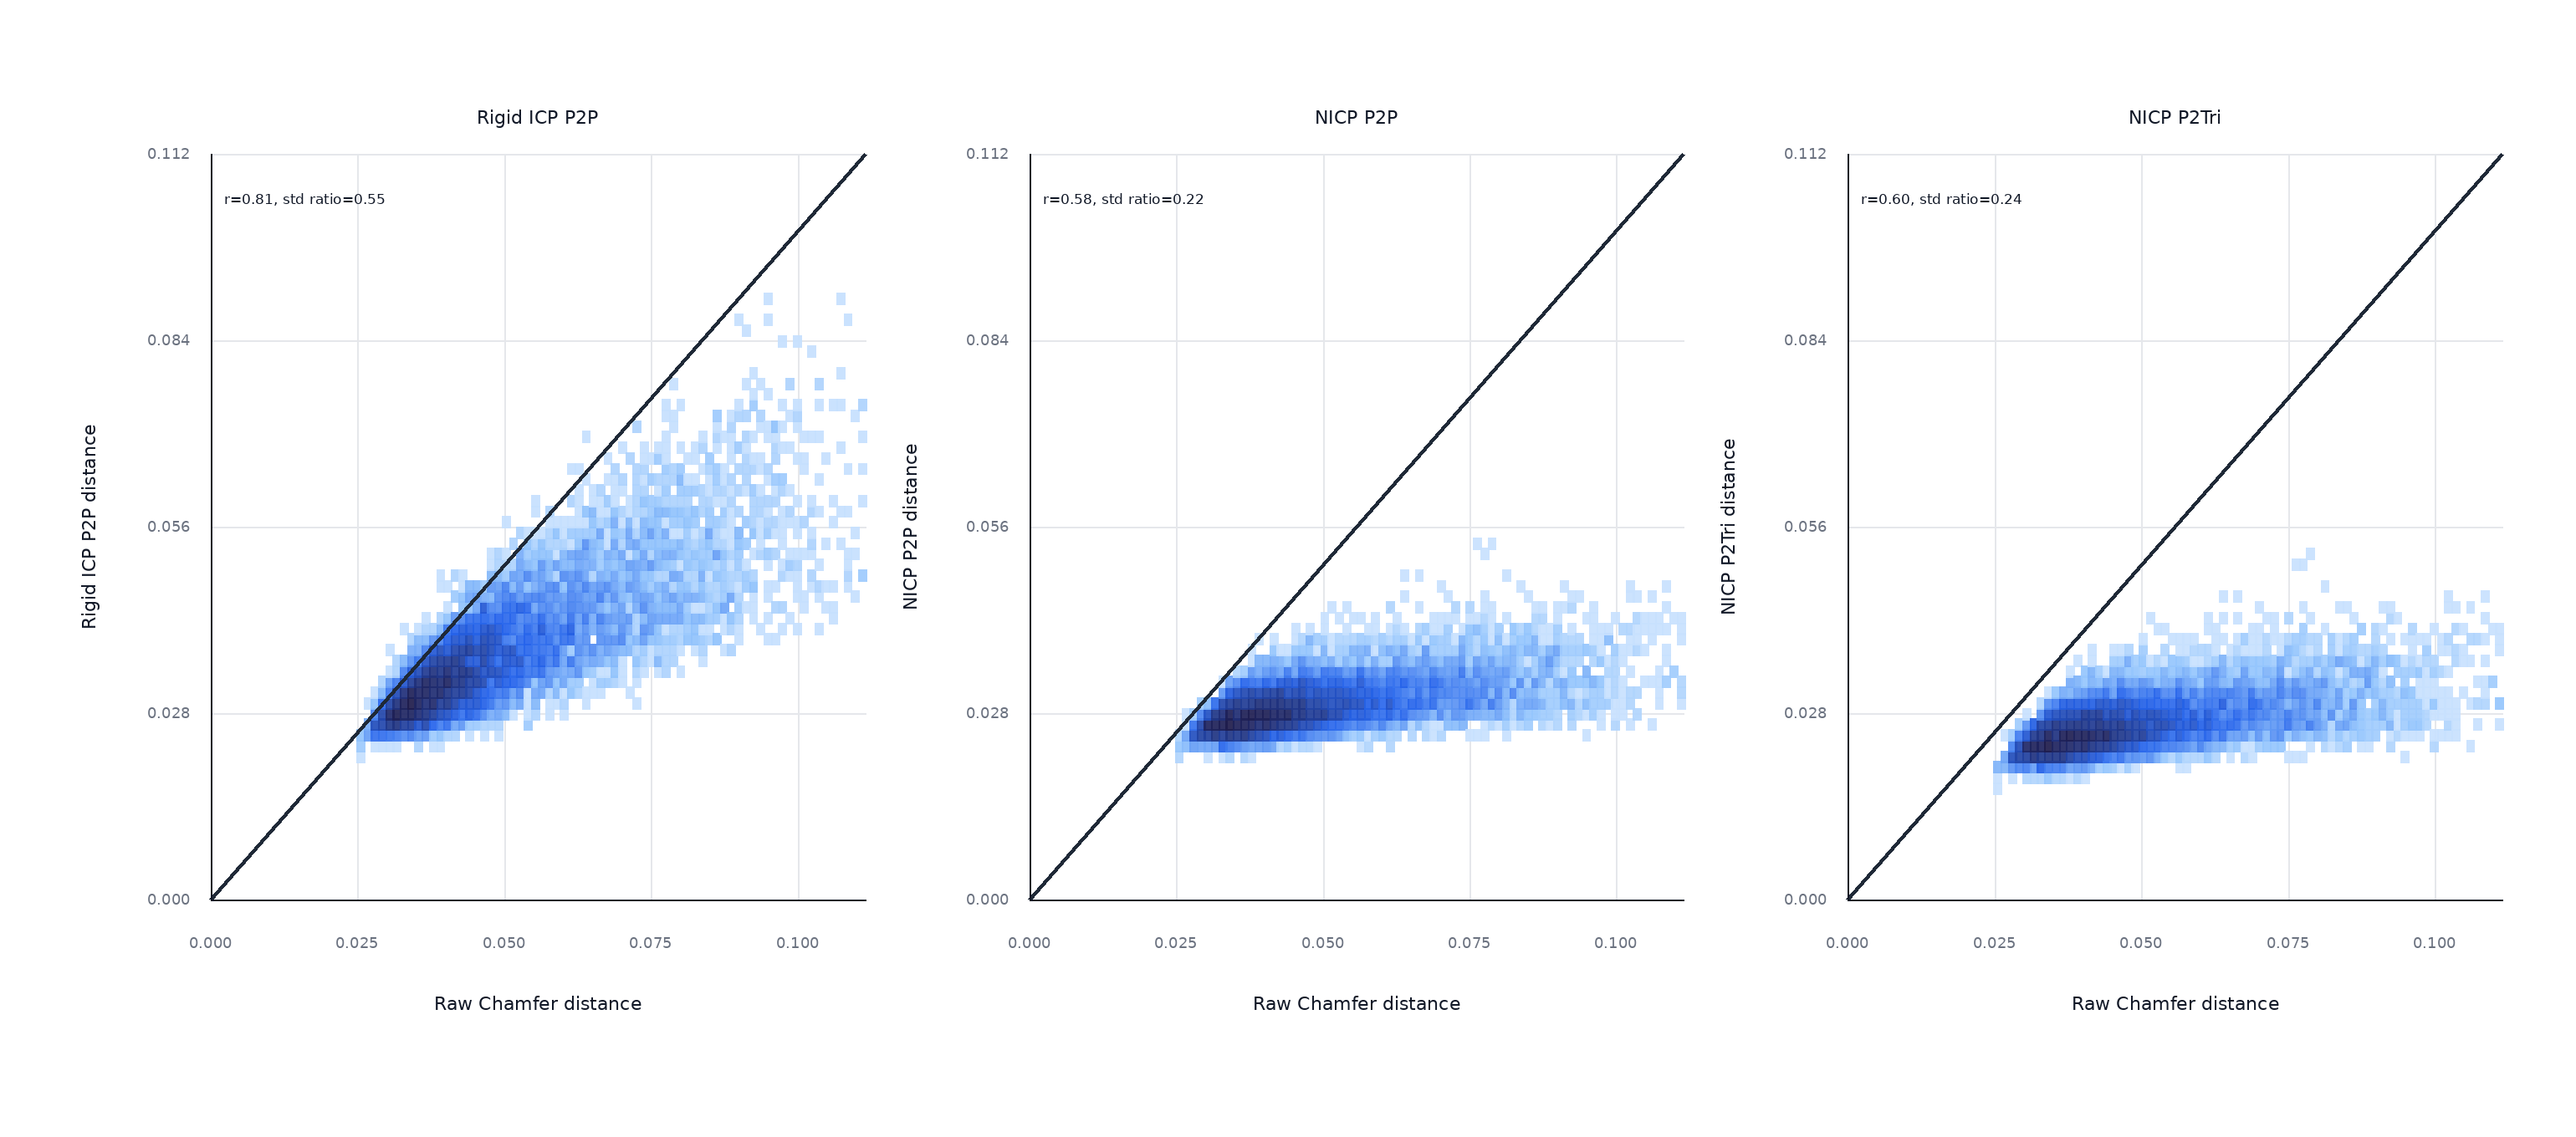
\includegraphics[width=0.85\textwidth]{imgs/raw_vs_registered_density_panels_shared_axes.png}
    \caption{Registration compresses the distance landscape. Each panel compares raw Chamfer distances with distances obtained after a registration-based pipeline on clean cross-topology mesh pairs. The diagonal indicates identity mapping, while the binned median shows that non-rigid ICP maps pairs with substantially different raw distances into a narrow registered-distance range.}
\label{fig:registration_distance_compression}
\end{figure*}

This compression is consistent with stronger geometric fitting reducing agreement with ground-truth identity rankings, but it does not prove the cause: Spearman correlation is invariant to any monotone compression of the distances, so a smaller spread alone does not lower it. The learned metric avoids this pair-specific fitting step by embedding all meshes into a shared space and comparing them with a single global distance function.

\subsubsection{Out-of-Distribution Transfer}
\label{sec:ood_transfer}
We finally evaluate transfer to FaceScape~\cite{facescape}, a separate mesh family unseen during REMESH training. The goal is not to claim universal zero-shot generalization, but to assess how much of the learned identity-ranking structure transfers beyond the source benchmark.

As shown in Table~\ref{tab:faceverse_summary}, in the full-neutral FaceScape setting, the REMESH-trained model shows nontrivial zero-shot transfer: on 110 neutral-pose subjects and 5,995 subject pairs, the latent distance reaches Spearman correlation $0.532$ in the clean setting. However, Chamfer remains stronger, reaching $0.605$. Under mixed perturbations, the gap increases, with latent Spearman $0.477$ compared with $0.638$ for Chamfer. Thus, the learned metric does not collapse out of domain, but it does not outperform Chamfer in this within-topology FaceScape setting.

The harder FaceScape cross-topology setting exposes a clearer limitation. When each subject is represented by both a downsampled FaceScape mesh and an independently remeshed 10k-vertex variant, zero-shot transfer is insufficient: the latent metric reaches only $0.115$ Spearman, compared with $0.598$ for Chamfer. This indicates that cross-topology transfer to a new mesh family is a substantial domain shift for the REMESH-trained model.

Few-shot FaceScape adaptation substantially improves this behavior. With 75 FaceScape fine-tuning identities and evaluation on 35 held-out subjects, the adapted model reaches $0.537$ Spearman in the clean cross-topology setting, outperforming Chamfer at $0.403$. It also remains stronger under translation with $\sigma=0.10$ ($0.486$ vs. $0.417$). These results suggest that the FaceScape gap is primarily a domain-shift issue rather than a fundamental failure of the learned metric, although robustness under stronger jitter remains limited. Full FaceScape adaptation and forgetting results are reported in
Appendix~\ref{app:faceverse_adaptation}.

\begin{table}[!ht]
\centering
\footnotesize
\caption{Zero-shot transfer on FaceScape is nontrivial in the within-topology full-neutral setting, insufficient in the harder cross-topology setting, and improves after few-shot target-domain adaptation.}
\label{tab:faceverse_summary}
\begin{tabular}{lccc}
\toprule
Setting & Latent & Chamfer & $\Delta$ \\
\midrule
Full-neutral zero-shot, clean & 0.532 & 0.605 & -0.073 \\
Full-neutral zero-shot, mixed & 0.477 & 0.638 & -0.161 \\
Cross-topology zero-shot, clean & 0.115 & 0.598 & -0.483 \\
75-shot cross-topology, clean & \textbf{0.537} & 0.403 & +0.134 \\
75-shot cross-topology, trans. 0.10 & \textbf{0.486} & 0.417 & +0.069 \\
\bottomrule
\end{tabular}
\end{table}


\subsubsection{Extended Baselines (Held-Out)}
\label{sec:extended_baselines}
Table~\ref{tab:extended_baselines} compares the registration-free baselines of Sect.~\ref{sec:baseline_protocol} on the 100 held-out REMESH identities. The cross-topology column of Sect.~\ref{sec:xtopo_results} (no crop) is split into pairs that differ only in tessellation (12 ordered topology pairs) and pairs that involve the noisy variant (8). Varifold and currents are computed at full resolution with the measure normalized to unit mass in the max-abs frame, so that meshes with different areas are comparable.

\begin{table*}[!ht]
\centering
\footnotesize
\caption{Extended baselines on the held-out REMESH split: Spearman correlation ($\uparrow$) with $D_{\mathrm{GT}}$, 95\% subject-level bootstrap CIs in brackets. Bold: best non-control row per column. The bounding-box proxy (centre and diagonal of the per-mesh-normalized mesh) is a control, not a shape metric.}
\label{tab:extended_baselines}
\setlength{\tabcolsep}{3pt}
\begin{tabular}{lcccc}
\toprule
Method & Same topology & Cross, no crop & Tessellation only & Perturbation only \\
\midrule
Chamfer & 0.644 [0.580, 0.707] & \textbf{0.469 [0.399, 0.532]} & 0.454 [0.383, 0.519] & \textbf{0.502 [0.431, 0.566]} \\
Varifold (unit mass) & 0.646 [0.576, 0.709] & 0.258 [0.213, 0.298] & \textbf{0.496 [0.427, 0.556]} & 0.307 [0.244, 0.370] \\
Currents (unit mass) & \textbf{0.663 [0.588, 0.726]} & 0.210 [0.153, 0.268] & 0.287 [0.205, 0.359] & 0.289 [0.226, 0.351] \\
LPIPS & 0.590 [0.507, 0.662] & 0.127 [0.097, 0.155] & 0.287 [0.228, 0.343] & 0.148 [0.092, 0.207] \\
ArcFace & 0.293 [0.222, 0.372] & 0.218 [0.161, 0.275] & 0.300 [0.228, 0.370] & 0.160 [0.092, 0.222] \\
CLIP & 0.358 [0.264, 0.449] & 0.087 [0.057, 0.118] & 0.226 [0.159, 0.296] & 0.039 [$-$0.048, 0.128] \\
DINOv2 & 0.378 [0.275, 0.477] & 0.058 [0.032, 0.089] & 0.147 [0.097, 0.203] & 0.034 [$-$0.059, 0.130] \\
\midrule
BBox proxy (control) & 0.284 [0.194, 0.369] & 0.117 [0.076, 0.162] & 0.088 [0.051, 0.127] & 0.167 [0.111, 0.220] \\
Learned metric & \todo{final model} & \todo{} & \todo{} & \todo{} \\
\bottomrule
\end{tabular}
\end{table*}

Chamfer remains the best baseline whenever topology changes: in the no-crop cross-topology column it reaches $0.469$, against $0.258$ for the unit-mass varifold and at most $0.218$ for every other baseline. The varifold overtakes Chamfer only when the change is purely one of tessellation ($0.496$ vs.\ $0.454$, with overlapping CIs), and falls to $0.307$ under perturbation. In the same-topology column the three geometric distances are statistically indistinguishable ($0.644$--$0.663$). The bounding-box control is informative for the perceptual baselines: in the no-crop cross-topology column and under perturbation, CLIP ($0.087$, $0.039$) and DINOv2 ($0.058$, $0.034$) do not exceed a proxy that sees only the position and size of the bounding box ($0.117$, $0.167$); they exceed it only in the tessellation-only column. Learned-metric row: \todo{held-out numbers of the final model, not yet decided}.

\subsubsection{Reconstruction Methods on Real Scans (Multiface)}
\label{sec:multiface_recon}
We rank 3DDFA\_V2, SynergyNet and PRNet on 13 Multiface subjects (3,075 reconstructions per method) under three criteria (Sect.~\ref{sec:ref_sets}): similarity-ICP point-to-surface distance, Chamfer distance on a patch equal to the ground-truth one, and our latent distance. Table~\ref{tab:multiface_recon} reports the resulting rankings and the per-subject Kendall $\tau$ with subject-level bootstrap CIs.

\begin{table*}[!ht]
\centering
\footnotesize
\caption{Reconstruction methods on Multiface (13 subjects). (a) Per-criterion score (lower is better; mean over subjects of the per-subject median) and resulting order. (b) Per-subject Kendall $\tau$ between criteria, 95\% subject-level bootstrap CI. Under independent rankings $\tau$ has mean 0 and s.d.\ 0.177, and 16.7\% of subjects have identical order. Split-half reliability within a criterion: 0.86--0.98.}
\label{tab:multiface_recon}
\setlength{\tabcolsep}{3pt}
\begin{tabular}{lcccl}
\toprule
\multicolumn{5}{l}{\textbf{(a) Rankings}}\\
Criterion & 3DDFA\_V2 & PRNet & SynergyNet & Order \\
\midrule
Similarity-ICP p2s (mm) & 1.242 & 1.260 & 1.519 & 3DDFA $<$ PRNet $<$ Syn. \\
Chamfer, equal patch (mm) & 2.368 & 2.488 & 2.559 & 3DDFA $<$ PRNet $<$ Syn. \\
Learned (latent) & 0.721 & 0.919 & 0.749 & 3DDFA $<$ Syn. $<$ PRNet \\
\midrule
\multicolumn{5}{l}{\textbf{(b) Agreement between criteria}}\\
Criteria & \multicolumn{2}{c}{Kendall $\tau$ [95\% CI]} & \multicolumn{2}{c}{Identical order} \\
\midrule
ICP vs.\ Chamfer (equal patch) & \multicolumn{2}{c}{0.80 [0.59, 0.95]} & \multicolumn{2}{c}{69\% of subjects} \\
ICP vs.\ Chamfer (mm, ICP scale) & \multicolumn{2}{c}{0.85 \todo{CI}} & \multicolumn{2}{c}{--} \\
ICP vs.\ learned & \multicolumn{2}{c}{$-$0.03 [$-$0.28, 0.18]} & \multicolumn{2}{c}{0\%} \\
Chamfer (equal patch) vs.\ learned & \multicolumn{2}{c}{0.18 [$-$0.08, 0.44]} & \multicolumn{2}{c}{--} \\
Chamfer (mm, ICP scale) vs.\ learned & \multicolumn{2}{c}{0.13 \todo{CI}} & \multicolumn{2}{c}{--} \\
\bottomrule
\end{tabular}
\end{table*}

At equal support and scale, the geometric criteria with and without ICP agree ($\tau=0.80$, identical order for 69\% of subjects): on real reconstructions, alignment does not change the ranking of the methods. The learned metric disagrees with all of them ($\tau=0.13$--$0.18$ against Chamfer, $-0.03$ against ICP, all within about one standard deviation, $0.177$, of chance), and this disagreement is reliable rather than noise (split-half reliability $0.92$ for the learned metric). It ranks PRNet last, where the geometric criteria rank SynergyNet last. Without an external identity reference we cannot say which ranking is right. We therefore report this as a negative result: Multiface does not support the claim that alignment distorts the ranking of reconstruction methods, which rests here on synthetic data and the crop control (Sect.~\ref{sec:ref_sets}), and it is a limit of our evidence on real scans. We do not test whether the disagreement stems from the encoder reading per-mesh-normalized, unclipped reconstructions. \todo{final tau table with CIs for all pairs exported to a result file}

\subsubsection{Expressions}
\label{sec:expressions}
We test robustness to expression on the 100 held-out ICT identities, each with 5 random expression vectors per subject (3--8 active blendshapes out of 45, coefficients 0.3--1.0, gaze excluded), so that expressions perturb each identity differently. Spearman correlation is computed against the neutral $D_{\mathrm{GT}}$ with the area-normalized BFM-trained model (seed 1234); Table~\ref{tab:expressions} gives three regimes.

\begin{table*}[!ht]
\centering
\small
\caption{Spearman correlation ($\uparrow$) with the neutral $D_{\mathrm{GT}}$ on 100 held-out ICT subjects, under per-subject random expressions (BFM-trained model, seed 1234). $\Delta$: change from the neutral-vs-neutral reference. 95\% subject-level bootstrap CIs.}
\label{tab:expressions}
\setlength{\tabcolsep}{4pt}
\begin{tabular}{lcccc}
\toprule
Regime & Latent & $\Delta$ & Chamfer & $\Delta$ \\
\midrule
Neutral vs.\ neutral & 0.841 & -- & 0.951 & -- \\
Expression vs.\ neutral & 0.784 [0.727, 0.831] & $-$0.056 & 0.914 [0.884, 0.938] & $-$0.036 \\
Mixed expressions & 0.739 [0.680, 0.790] & $-$0.101 & 0.886 [0.846, 0.917] & $-$0.065 \\
\bottomrule
\end{tabular}
\end{table*}

Expressions degrade the identity ranking for both distances, and the learned metric suffers more than Chamfer (mixed regime: $-0.101$ vs.\ $-0.065$; expression-vs-neutral: $-0.056$ vs.\ $-0.036$; point estimates, \todo{paired CI on the difference of drops}). This is expected: the model is trained on neutral BFM faces only. \todo{ICT-trained and joint models}

\subsubsection{Cross-3DMM Transfer}
\label{sec:cross3dmm}
In the zero-shot BFM$\rightarrow$ICT transfer (three BFM-trained models, 100 held-out ICT identities, mesh-pair protocol), the latent distance reaches Spearman $0.30$ ($0.29/0.31/0.30$ over the three seeds) against $0.44$ for Chamfer: a model trained on a single 3DMM does not transfer to a second one, and the learned metric loses to Chamfer. \todo{table: BFM-only / ICT-only / joint $\times$ BFM / ICT}

\subsection{Additional Dataset and Implementation Details}
\label{app:implementation_details}

\subsubsection{REMESH Construction Details}
\label{app:remesh_details}

The main REMESH construction protocol is described in
Sec.~\ref{sec:remesh_benchmark}. Here we provide additional implementation
details and a qualitative visualization of the resulting topology variants.

The GT-ready source dataset contains 4,999 full-resolution synthetic meshes, each
with 53,215 vertices and 105,954 faces. After canonical facial-region extraction,
each cropped canonical mesh contains 23,470 vertices and 46,440 faces. The
generated REMESH variants have the following approximate resolutions: Remesh,
16.5k vertices and 32.5k faces; Crop, 21k vertices and 41.5k faces; Down8k,
8.1k vertices and 16k faces; and Up60k, 60.4k vertices and 120k faces.

Renders of REMESH examples are omitted (BFM license).

% figura fig:remesh_synthetic_examples_app tolta (render di mesh BFM, licenza)


\subsubsection{Identity Distinctness Between Training and Held-Out Splits}
\label{app:identity_distinctness}
Because REMESH identities are sampled from the same 3D morphable model, we
must verify that no held-out identity is a near-duplicate of a training
identity. For each held-out subject $h$ we compute the distance to its nearest
training subject, $m_h=\min_t d(h,t)$, and compare it with (i) the distribution
of distances between held-out subjects and (ii) the nearest-neighbour distance
of each training subject within the training set (leave-one-out). The second
reference is the appropriate one, because $m_h$ is itself a minimum over
hundreds (BFM) or thousands (ICT) of candidates. The BFM shape coefficients of
the 500 REMESH identities were not retained, so for BFM we use $D_{\mathrm{GT}}$
(vertex-mean $L_2$ on the normalized meshes); for ICT we use both
$D_{\mathrm{GT}}$ and the Euclidean distance between identity weights (100 PCA
modes, in units of standard deviation). Splits are those of the trained models
(BFM, seed 1234: 400/100; ICT-only: 4000/1000).

On BFM, the smallest $m_h$ is 0.156, i.e.\ 0.47 times the median
held-out--held-out distance (0.336; 1st and 5th percentiles 0.208 and 0.239);
the median $m_h$ (0.193) matches the median leave-one-out nearest-neighbour
distance within training (0.196), and no held-out subject is closer to the
training set than the closest training pair (0.131). On ICT, the smallest $m_h$
is 0.29 times the median held-out--held-out distance in $D_{\mathrm{GT}}$ (0.067
vs.\ 0.228; percentiles 1 and 5: 0.118, 0.140) and 0.64 times in weight space
(8.96 vs.\ 14.06; 11.78, 12.43); the median $m_h$ equals the training
leave-one-out median in both spaces (0.096 vs.\ 0.096; 11.04 vs.\ 11.05), and
1--2\% of held-out subjects fall below its 1st percentile, as expected by
chance. Most $m_h$ lie below the 1st percentile of held-out--held-out distances
(73\% on BFM, 92--93\% on ICT), but this is the expected effect of a minimum over
many candidates and holds equally for training subjects among themselves. No
held-out identity is a near-duplicate of a training identity; the same holds
for the BFM splits of seeds 2345 and 3456 and for the joint model's split.

\subsubsection{DiffusionNet Operators}
\label{app:diffusionnet_operators}
For every mesh realization, we precompute the surface operators required by DiffusionNet, including the mass matrix, Laplace--Beltrami operator, spectral eigensystem, and tangent gradient operators. Vertex coordinates encode the extrinsic position of the surface in $\mathbb{R}^3$, whereas the Laplace--Beltrami operators encode intrinsic surface geometry.

Under a rigid motion $T(x)=Rx+t$, with $R\in SO(3)$ and $t\in\mathbb{R}^3$, intrinsic distances, angles, and area elements on the continuous surface are preserved. Consequently, the continuous Laplace--Beltrami operator and its spectrum are invariant to global rotations and translations:
\begin{equation}
\Delta_{T(\mathcal{M})}=\Delta_{\mathcal{M}},
\qquad
\Delta_{\mathcal{M}}\phi_\ell=\lambda_\ell\phi_\ell.
\end{equation}
This provides a useful geometric bias for robustness to global pose changes.

However, topology changes still affect the discrete operators. Remeshing,
decimation, subdivision, cropping, and noise modify the sampled mesh and
therefore change the discrete mass matrix, Laplacian, eigenbasis, and gradient
operators. Thus, intrinsic operators do not guarantee topology invariance by
themselves. Our model combines extrinsic XYZ coordinates with geometry-aware
diffusion operators and is explicitly trained across topology variants, so that
topology-dependent operator differences are treated as nuisance variation while
identity-related geometric differences are preserved. Our evaluation pairs meshes
across remeshing, decimation, noise and upsampling (Sect.~\ref{M-sec:hifi});
boundary crops, although in the training distribution, break the embedding
(Sect.~\ref{M-sec:limitations}).
% NOTA (11 ott, critic): "This holds for remeshing..." tolto: la robustezza alla discretizzazione non ha ancora un
% numero dedicato (media dentro le coppie di topologie senza crop, emendamento 3).

\subsubsection{Training Details}
\label{app:training_details}

The reported model uses the \texttt{xyz\_dn} encoder with latent dimension 256,
hidden width 128, four DiffusionNet blocks, dropout 0.1, and mean--max pooling.
Training uses mini-batches of 5 subjects with up to 6 mesh realizations per
subject. The model is trained for 120 epochs with learning rate $10^{-4}$,
weight decay $10^{-6}$, and gradient clipping at 1.0.

The training objective is defined in Sec.~\ref{sec:training_objective}. In all
reported experiments we use $\lambda_{\mathrm{subj}}=1$,
$\lambda_{\mathrm{mesh}}=1$, $\lambda_r=0.5$, and $\lambda_i=0.25$.

Mesh-level supervision uses cross-topology pairs only. Ranking losses sample
1024 constraints per batch, with margin $\gamma=0.05$, tolerance $\tau=0.02$,
and 70\% hard constraints.

During training, online perturbations are applied with probability 0.6. The
perturbation modes are translation, rotation, and jitter, sampled with relative
weights $4{:}2{:}1$. Jitter magnitude is sampled log-uniformly between
$5\times10^{-4}$ and $2\times10^{-2}$. Rotations use angles between
$0.5^\circ$ and $12^\circ$, and translations use per-axis standard deviation
between $0.001$ and $0.03$.
\subsubsection{Mesh-Level Ranking Loss}
\label{app:mesh_level_ranking_loss}

At the mesh level, we compare two valid mesh pairs $a$ and $b$ and enforce the
ordering induced by their corresponding subject-level ground-truth distances:
\begin{equation}
\begin{split}
\mathcal L^{\mathrm{mesh}}_{\mathrm{rank}}
={}&
\mathbb E_{(a,b)}
\Big[
\max
\Big(
0,\;
\gamma
\\
&-
\operatorname{sign}
\left(
D_{\mathrm{GT}}^a-D_{\mathrm{GT}}^b
\right)
\left(
d_z^a-d_z^b
\right)
\Big)
\Big],
\end{split}
\end{equation}
where $d_z^a$ and $d_z^b$ are the latent distances of the two mesh pairs. We
ignore comparisons whose ground-truth distance difference is below $\tau=0.02$.

The identity-consistency term used in the main objective is
\begin{equation}
\mathcal L_{\mathrm{id}}
=
\frac{1}{|\mathcal S|}
\sum_{s\in\mathcal S}
\frac{1}{M_s}
\sum_{m=1}^{M_s}
\left\|
z_{s,m}-\bar z_s
\right\|_2^2 .
\end{equation}

\subsection{Cross-Topology Bootstrap Confidence Intervals}
\label{app:xtopo_bootstrap_ci}

Tables~\ref{tab:xtopo_chamfer_ci_app} and~\ref{tab:xtopo_latent_ci_app}
report 95\% subject-level bootstrap confidence intervals for the clean
same-topology and cross-topology ranking experiment. Each cell reports Spearman
correlation with $D_{\mathrm{GT}}$, followed by the 95\% confidence interval in
brackets. Confidence intervals are computed over 1,000 subject-level bootstrap
replicates, using the same procedure described in Sec.~\ref{sec:alignment_results}.

\begin{table*}[!htbp]
\centering
\scriptsize
\caption{
Raw Chamfer clean same-topology and cross-topology Spearman correlation with
95\% subject-level bootstrap confidence intervals. Rows indicate source topology
and columns indicate target topology.
}
\label{tab:xtopo_chamfer_ci_app}
\setlength{\tabcolsep}{2.0pt}
\renewcommand{\arraystretch}{1.08}
\resizebox{\textwidth}{!}{%
\begin{tabular}{lcccccc}
\toprule
Source & crop & down8k & noisy & original & remesh & up60k \\
\midrule
crop & 0.558 [0.480, 0.632] & -0.093 [-0.212, 0.034] & -0.048 [-0.165, 0.072] & -0.035 [-0.146, 0.091] & -0.008 [-0.132, 0.112] & -0.074 [-0.198, 0.049] \\
down8k & 0.037 [-0.095, 0.174] & 0.743 [0.687, 0.792] & 0.472 [0.393, 0.551] & 0.407 [0.310, 0.491] & 0.436 [0.344, 0.519] & 0.611 [0.528, 0.682] \\
noisy & 0.083 [-0.030, 0.204] & 0.313 [0.216, 0.401] & 0.739 [0.674, 0.794] & 0.659 [0.586, 0.724] & 0.579 [0.498, 0.649] & 0.489 [0.406, 0.567] \\
original & 0.093 [-0.014, 0.211] & 0.240 [0.154, 0.328] & 0.627 [0.551, 0.698] & 0.729 [0.667, 0.790] & 0.553 [0.472, 0.624] & 0.414 [0.327, 0.496] \\
remesh & 0.102 [-0.005, 0.218] & 0.338 [0.255, 0.431] & 0.621 [0.541, 0.691] & 0.622 [0.544, 0.691] & 0.709 [0.647, 0.763] & 0.525 [0.444, 0.605] \\
up60k & 0.061 [-0.067, 0.184] & 0.564 [0.479, 0.644] & 0.597 [0.518, 0.669] & 0.539 [0.463, 0.608] & 0.573 [0.497, 0.643] & 0.735 [0.674, 0.791] \\
\bottomrule
\end{tabular}
}
\end{table*}

\begin{table*}[!htbp]
\centering
\scriptsize
\caption{
Latent distance clean same-topology and cross-topology Spearman correlation with
95\% subject-level bootstrap confidence intervals. Rows indicate source topology
and columns indicate target topology.
}
\label{tab:xtopo_latent_ci_app}
\setlength{\tabcolsep}{2.0pt}
\renewcommand{\arraystretch}{1.08}
\resizebox{\textwidth}{!}{%
\begin{tabular}{lcccccc}
\toprule
Source & crop & down8k & noisy & original & remesh & up60k \\
\midrule
crop & 0.831 [0.789, 0.866] & 0.668 [0.603, 0.730] & 0.737 [0.672, 0.791] & 0.760 [0.696, 0.811] & 0.658 [0.591, 0.720] & 0.687 [0.615, 0.747] \\
down8k & 0.692 [0.619, 0.751] & 0.883 [0.847, 0.909] & 0.793 [0.741, 0.839] & 0.781 [0.724, 0.829] & 0.795 [0.746, 0.836] & 0.804 [0.746, 0.847] \\
noisy & 0.747 [0.684, 0.802] & 0.779 [0.722, 0.825] & 0.900 [0.874, 0.923] & 0.821 [0.771, 0.864] & 0.771 [0.720, 0.816] & 0.791 [0.737, 0.837] \\
original & 0.771 [0.715, 0.821] & 0.772 [0.717, 0.816] & 0.822 [0.774, 0.865] & 0.902 [0.873, 0.925] & 0.762 [0.712, 0.806] & 0.787 [0.741, 0.829] \\
remesh & 0.685 [0.615, 0.740] & 0.796 [0.742, 0.840] & 0.784 [0.729, 0.833] & 0.771 [0.716, 0.818] & 0.873 [0.838, 0.900] & 0.806 [0.751, 0.848] \\
up60k & 0.705 [0.631, 0.766] & 0.798 [0.744, 0.844] & 0.798 [0.744, 0.843] & 0.788 [0.728, 0.834] & 0.801 [0.755, 0.845] & 0.890 [0.860, 0.917] \\
\bottomrule
\end{tabular}
}
\end{table*}

\subsection{Additional Perturbation Results}

\label{app:perturbations}


\subsubsection{Selected Cross-Topology Pairs}
\label{app:selected_topology_pairs}

Table~\ref{tab:xtopo_latent_chamfer_app} reports cross-topology Spearman
correlation across perturbation regimes for representative ordered topology
pairs. Each entry reports latent distance / raw Chamfer. On REMESH with the legacy
maxabs reference (v1 model, fb100; Sect.~\ref{sec:heldout_contamination}), Chamfer
is highly sensitive to topology and support mismatch, while the learned metric
keeps a stronger agreement with the reference ranking. This in-domain result does
not carry over to held-out families, where boundary crops break our current
encoder (Sect.~\ref{M-sec:limitations}).
% SMENTITO (11 ott) fuori dominio per le coppie col crop: vale solo per il modello v1 su REMESH (GT maxabs). Vedi
% Sect. sec:limitations. Tolto "confirm the trend observed in the main paper" (critic, 11 ott).

\begin{table*}[h]
\centering
\small
\caption{
Cross-topology Spearman correlation across perturbation regimes for selected
ordered topology pairs. Results are computed over 4,950 subject pairs per
topology pair. Each cell reports \textbf{Latent / Chamfer}. Higher is better.
}
\label{tab:xtopo_latent_chamfer_app}
\begin{tabular}{lccccc}
\toprule
Topology Pair & Clean & Jitter & Translation & Rotation & Mixed \\
\midrule
crop $\rightarrow$ down8k
& 0.668 / -0.093
& 0.585 / -0.092
& 0.653 / -0.092
& 0.648 / -0.097
& 0.557 / -0.093 \\

crop $\rightarrow$ remesh
& 0.658 / -0.008
& 0.564 / -0.014
& 0.647 / 0.005
& 0.632 / -0.013
& 0.518 / -0.021 \\

crop $\rightarrow$ up60k
& 0.687 / -0.074
& 0.628 / -0.070
& 0.672 / -0.069
& 0.650 / -0.081
& 0.569 / -0.073 \\

down8k $\rightarrow$ noisy
& 0.793 / 0.472
& 0.692 / 0.495
& 0.781 / 0.453
& 0.769 / 0.465
& 0.681 / 0.461 \\

down8k $\rightarrow$ up60k
& 0.804 / 0.611
& 0.732 / 0.576
& 0.789 / 0.598
& 0.758 / 0.579
& 0.695 / 0.544 \\

original $\rightarrow$ remesh
& 0.762 / 0.553
& 0.674 / 0.549
& 0.753 / 0.546
& 0.737 / 0.545
& 0.640 / 0.497 \\

remesh $\rightarrow$ up60k
& 0.806 / 0.525
& 0.755 / 0.532
& 0.788 / 0.531
& 0.758 / 0.492
& 0.688 / 0.506 \\
\bottomrule
\end{tabular}
\end{table*}

\subsubsection{Full Registration Pipeline Under Perturbations}
\label{app:facebench_pipeline_perturbations}

We further compare the proposed latent distance against the full FaceBench
geometry pipeline under perturbations. This benchmark includes raw Chamfer,
rigid ICP point-to-point distance, and non-rigid ICP distances computed as
point-to-point and point-to-triangle errors. Unlike the cross-topology breakdown
in the main paper, this experiment evaluates complete registration pipelines
rather than raw Chamfer alone.

\begin{table*}[h]
\centering
\small
\caption{
FaceBench pipeline comparison under perturbations. Each cell reports Spearman /
Pearson correlation with the ground-truth identity distance. Bold indicates the
best score. Higher is better.
}
\label{tab:facebench_pipeline_perturbed_app}
\begin{tabular}{lcccc}
\toprule
Method & Clean & Translation 0.10 & Rotation 0.10 & Jitter 0.10 \\
\midrule
Latent distance
& \textbf{0.786} / \textbf{0.816}
& \textbf{0.770} / \textbf{0.795}
& \textbf{0.765} / \textbf{0.802}
& \textbf{0.562} / \textbf{0.597} \\

Raw Chamfer
& 0.345 / 0.388
& 0.343 / 0.387
& 0.337 / 0.377
& 0.258 / 0.312 \\

Rigid ICP P2P
& 0.383 / 0.468
& 0.372 / 0.465
& 0.379 / 0.464
& -0.028 / 0.004 \\

NICP P2P
& 0.276 / 0.364
& 0.246 / 0.340
& 0.254 / 0.348
& -0.005 / 0.026 \\

NICP P2Tri
& 0.276 / 0.361
& 0.245 / 0.337
& 0.255 / 0.346
& 0.067 / 0.100 \\
\bottomrule
\end{tabular}
\end{table*}

% NOTA (11 ott): in dominio (REMESH, GT maxabs, baseline normalizzate per maxabs). Con la GT FR e le baseline in mm
% il quadro cambia (aau/runs/evidence/e12/summary.md, sez. 5; Sect. sec:factorized_results).
On REMESH with the legacy maxabs reference, across clean, translation, rotation,
and jitter perturbations, the learned latent distance remains more correlated
with the reference identity distance than all geometry-only baselines. The gap
is particularly pronounced under jitter, where rigid and non-rigid registration
become nearly uncorrelated with identity ranking, while the latent distance still
preserves a Spearman correlation of $0.562$. With the form reference and
size-preserving baselines on held-out families the picture changes
(Sect.~\ref{M-sec:limitations}).

\subsection{Additional Registration Compression Analysis}
\label{app:compression_analysis}

Figure~\ref{fig:distance_compression_boxplot_app} reports the distribution of
clean cross-topology geometric distances before and after registration. The
boxplot complements the distance-compression statistics reported in the main
paper. Compared with raw Chamfer, rigid ICP and especially non-rigid ICP reduce
the spread of inter-subject distances, supporting the hypothesis that
registration can suppress identity-discriminative variation.

\begin{figure}[h]
    \centering
    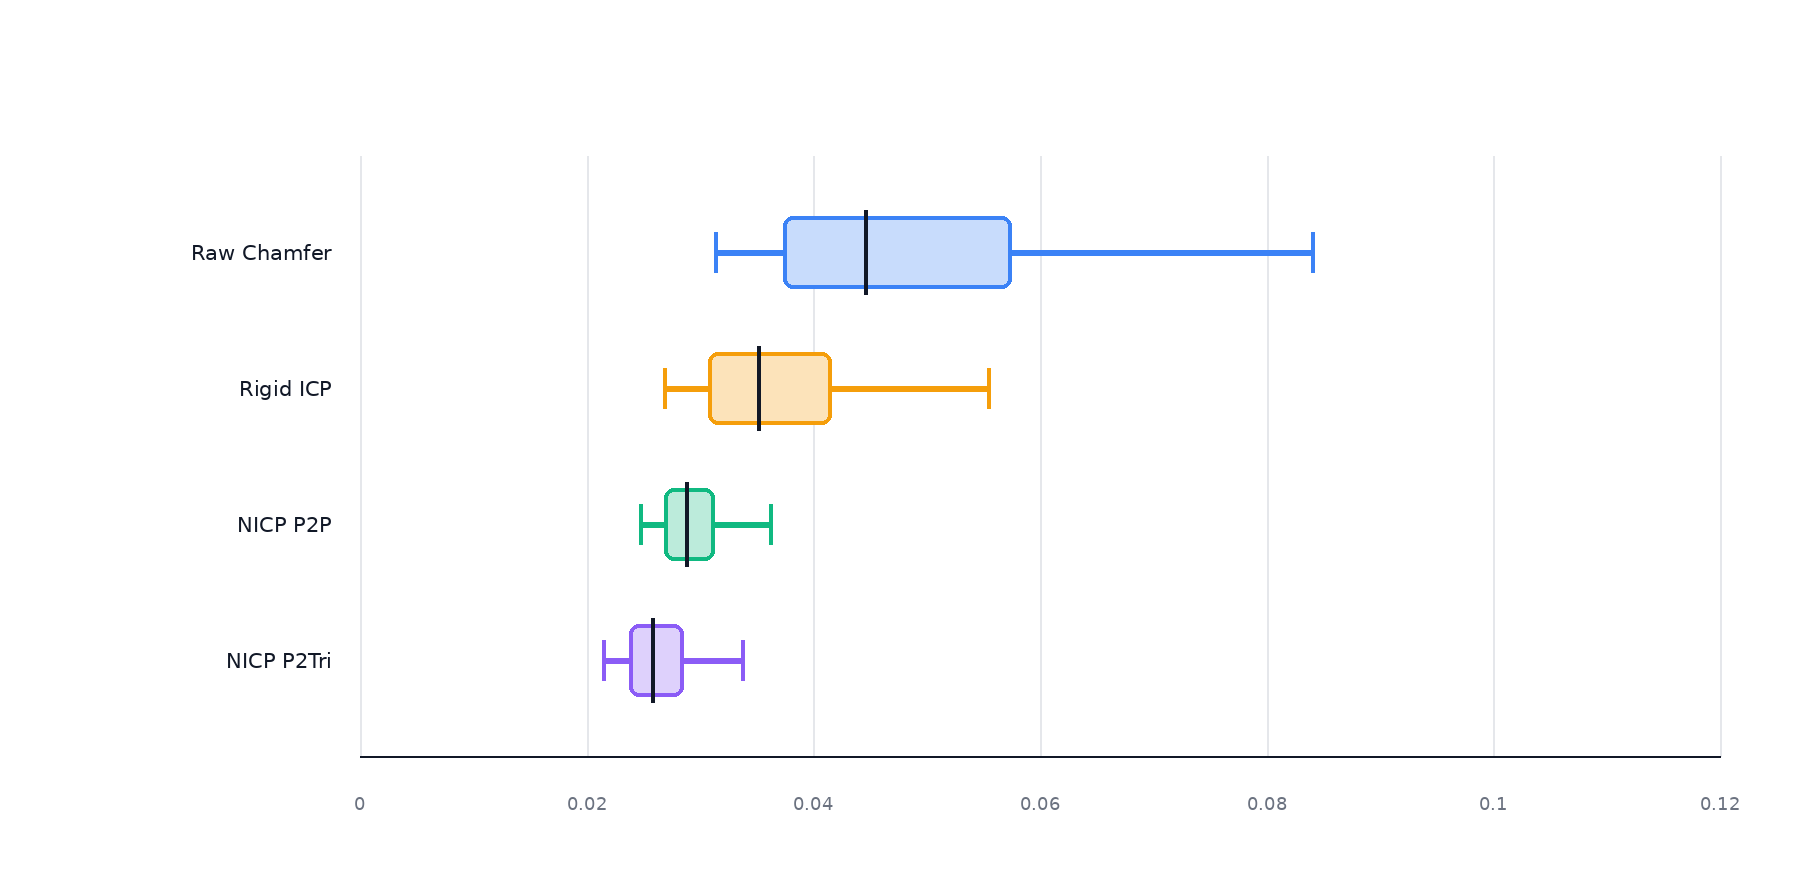
\includegraphics[width=0.85\linewidth]{imgs/clean_geometry_distance_boxplot.png}
    \caption{
    Distribution of clean cross-topology geometric distances before and after
    registration. Compared with raw Chamfer, rigid ICP and especially non-rigid
    ICP substantially reduce the spread of inter-subject distances.
    }
    \label{fig:distance_compression_boxplot_app}
\end{figure}

We observe the same trend under translation and rotation perturbations. Rigid ICP
consistently reduces the interquartile range to approximately 59--63\% of raw
Chamfer, while non-rigid ICP reduces it to approximately 18--20\%. Under jitter,
all geometric distances are affected by local noise, but the clean and rigid
perturbation settings show that registration itself can remove substantial
inter-subject variation.

\subsection{FaceScape Adaptation and Forgetting}
\label{app:faceverse_adaptation}

\subsubsection{FaceScape Target-Domain Construction}
\label{app:faceverse_construction}

FaceScape~\cite{facescape} is used as an external target domain to assess how the
REMESH-trained metric transfers to a mesh family unseen during source training.
No FaceScape identities are used for REMESH training, checkpoint selection, or
hyperparameter tuning.

We consider two FaceScape evaluation settings. The first is a
\emph{full-neutral} setting, where each subject is represented by one neutral-pose
mesh. We select files matching \texttt{*\_01.npz}, yielding 110 subjects and one
mesh per subject:
\begin{equation}
N_{\mathrm{subjects}} = 110,
\qquad
N_{\mathrm{pairs}} = \binom{110}{2} = 5995.
\label{eq:faceverse_subject_pairs}
\end{equation}
Each mesh has approximately 10k vertices and 20k faces, with DiffusionNet
operators precomputed. Pairwise latent distances are compared against a
FaceScape subject-level distance matrix computed from clean FaceScape detail
meshes using mean per-vertex Euclidean distance.

The second is a harder \emph{cross-topology} setting. Each FaceScape identity is
represented by two mesh realizations:
\begin{itemize}
    \item \textbf{Downsampled FaceScape}: the original FaceScape mesh reduced to
    approximately 10k vertices.
    \item \textbf{Remesh10k}: an independently remeshed version of the same
    subject, also with approximately 10k vertices.
\end{itemize}
Both variants include precomputed DiffusionNet operators. The downsampled
FaceScape meshes contain on average 10,152 vertices and 20,000 faces, while the
remeshed variants contain on average 10,113 vertices and 20,000 faces.

The remeshing pipeline samples points uniformly from the source surface,
estimates and orients normals, performs Poisson surface reconstruction, crops the
result using a scaled source bounding box, and finally applies quadric decimation
to obtain approximately 20,000 faces. This creates a two-realization
cross-topology FaceScape benchmark with 110 subjects, 220 mesh samples, 5,995
subject pairs, and 11,990 mesh pairs.

\subsubsection{FaceScape Perturbation and Chamfer Protocols}
\label{app:faceverse_perturbation_protocol}

We evaluate FaceScape robustness under five synthetic perturbation scenarios:
clean, jitter, translation, rotation, and mixed. For the fixed-noise experiment,
we use $\sigma=0.05$. Rotation uses a maximum angle of $1+20\sigma$ degrees,
giving $2^\circ$ at $\sigma=0.05$. Translation uses per-axis standard deviation
$0.002+0.05\sigma$, giving $0.0045$ at $\sigma=0.05$. The sigma sweep evaluates
\begin{equation}
\sigma \in \{0.00, 0.02, 0.05, 0.10, 0.15, 0.20\}.
\label{eq:faceverse_sigma_sweep}
\end{equation}

The Chamfer baseline is evaluated both without ICP and, in a separate protocol,
with post-perturbation ICP. The no-ICP protocol uses raw Chamfer distances
computed directly between the evaluated meshes. The ICP variant aligns each
perturbed pair before Chamfer computation using 2048 ICP points, maximum
correspondence distance 0.05, and 20 ICP iterations.

\subsubsection{Full-Neutral Zero-Shot Evaluation}
\label{app:faceverse_full_neutral}

We first evaluate the frozen REMESH-trained encoder on the full-neutral
FaceScape setting. This setting tests whether the learned metric transfers any
identity-ranking structure to a new mesh family when topology variation is not
introduced.

\begin{table}[h]
\centering
\footnotesize
\caption{
FaceScape full-neutral zero-shot evaluation. The REMESH-trained model transfers
nontrivial identity-ranking structure, but Chamfer remains stronger in this
within-topology setting.
}
\label{tab:faceverse_full_neutral_app}
\begin{tabular}{lccc}
\toprule
Scenario & Latent Spearman & Chamfer Spearman & $\Delta$ \\
\midrule
clean & 0.531864 & 0.605202 & -0.073337 \\
mixed & 0.476996 & 0.638449 & -0.161453 \\
\bottomrule
\end{tabular}
\end{table}

The latent metric achieves a clean Spearman correlation of $0.532$, indicating
nontrivial zero-shot transfer rather than out-of-domain collapse. However,
Chamfer remains stronger in this full-neutral within-topology setting, reaching
$0.605$ in the clean case and $0.638$ under mixed perturbations. Thus, this
experiment should be interpreted as evidence of partial transfer, not as a
zero-shot win for the learned metric.

\subsubsection{Cross-Topology Zero-Shot Evaluation}
\label{app:faceverse_xtopo_zeroshot}

We next evaluate zero-shot transfer in the harder FaceScape cross-topology
setting, where each subject is represented by both a downsampled FaceScape mesh
and an independently remeshed 10k-vertex variant. This introduces target-domain
topology variation that is not present in the full-neutral setting.

\begin{table}[h]
\centering
\footnotesize
\caption{
FaceScape cross-topology zero-shot evaluation. This setting exposes a strong
domain shift for the REMESH-trained latent metric.
}
\label{tab:faceverse_xtopo_zeroshot_app}
\begin{tabular}{lccc}
\toprule
Scenario & Latent Spearman & Chamfer Spearman & $\Delta$ \\
\midrule
clean & 0.114807 & 0.598032 & -0.483225 \\
\bottomrule
\end{tabular}
\end{table}

In this harder cross-topology setting, the zero-shot latent metric is
insufficient: Spearman correlation drops to $0.115$, while Chamfer reaches
$0.598$. This result should not be presented as a positive zero-shot outcome.
Instead, it shows that transferring cross-topology robustness from REMESH to a
different mesh family is a substantial domain-shift problem and motivates the
few-shot FaceScape adaptation experiments below.

\subsubsection{Few-Shot FaceScape Fine-Tuning}
\label{app:faceverse_finetuning}

To assess whether the FaceScape cross-topology gap is due to domain shift, we
fine-tune the REMESH-trained checkpoint on increasing numbers of FaceScape
identities. Fine-tuning is performed in the FaceScape cross-topology setting
using the FaceScape identity distance matrix as supervision. Evaluation uses
held-out subjects and subject-pair mean aggregation.

One representative 75-shot mixed-augmentation run uses 150 symlinked mesh
entries for fine-tuning and evaluates on 35 held-out subjects, 70 samples, and
1,190 subject pairs. Table~\ref{tab:faceverse_75shot_app} reports the strongest
stored held-out result from this branch.

\begin{table*}[h]
\centering
\small
\caption{
Representative 75-shot FaceScape held-out cross-topology evaluation. The adapted
model outperforms Chamfer in the clean setting and under moderate translation.
}
\label{tab:faceverse_75shot_app}
\begin{tabular}{lccc}
\toprule
Scenario & Latent Spearman & Chamfer Spearman & $\Delta$ \\
\midrule
clean & 0.537433 & 0.403222 & +0.134211 \\
translation $\sigma=0.10$ & 0.485680 & 0.416691 & +0.068990 \\
\bottomrule
\end{tabular}
\end{table*}

After few-shot target-domain adaptation, the learned metric becomes stronger than
Chamfer in the held-out FaceScape cross-topology setting. In the clean case, it
achieves Spearman correlation $0.537$ compared with $0.403$ for Chamfer. Under
moderate translation, it remains stronger, with $0.486$ versus $0.417$.

These results suggest that the weak zero-shot cross-topology performance is
primarily a domain-shift issue rather than a fundamental inability of the learned
metric to represent FaceScape geometry. However, the adapted model is not
uniformly robust: under stronger jitter perturbations, performance degrades and
Chamfer can overtake the learned metric. Thus, FaceScape adaptation improves
target-domain cross-topology ranking, but does not fully solve robustness to
local geometric noise.

\subsubsection{Source-Domain Forgetting After FaceScape Fine-Tuning}
\label{app:faceverse_forgetting}

Target-domain adaptation improves FaceScape performance, but may reduce the
source-domain invariances learned on REMESH. To assess this, we re-evaluate the
FaceScape-adapted checkpoints on the original REMESH clean cross-topology
protocol. The evaluation uses 100 held-out REMESH identities, 600 meshes, and
148,500 ordered mesh pairs. Since Chamfer does not depend on the learned
checkpoint, we only recompute the latent metric and compare it against the
pre-fine-tuning REMESH model.

\begin{table*}[h]
\centering
\small
\caption{
Source-domain performance after FaceScape fine-tuning. The table reports clean
REMESH cross-topology Spearman correlation before and after adapting to
FaceScape. The mean topology-pair score averages Spearman correlations across
ordered topology pairs. Lower post-fine-tuning scores indicate source-domain
forgetting.
}
\label{tab:faceverse_finetune_forgetting_app}
\begin{tabular}{lccc}
\toprule
Model & Overall Spearman & Mean topology-pair Spearman & $\Delta$ mean \\
\midrule
Pre fine-tune REMESH & \textbf{0.751} & \textbf{0.764} & -- \\
FaceScape shot75 clean-biased & 0.595 & 0.637 & -0.128 \\
FaceScape shot75 mixed-augmentation & 0.519 & 0.587 & -0.177 \\
\bottomrule
\end{tabular}
\end{table*}

The results show clear source-domain forgetting. The clean-biased FaceScape
checkpoint drops from $0.764$ to $0.637$ mean topology-pair Spearman, while the
mixed-augmentation checkpoint drops further to $0.587$. This indicates that
FaceScape adaptation improves target-domain behavior but does not preserve the
full cross-topology robustness learned on REMESH.

To localize where forgetting occurs, we compute the relative percentage drop for
each ordered topology pair:
\begin{equation}
\mathrm{Drop}_{A \rightarrow B}
=
\frac{
\rho_{\mathrm{pre}}(A \rightarrow B)
-
\rho_{\mathrm{post}}(A \rightarrow B)
}{
\rho_{\mathrm{pre}}(A \rightarrow B)
}
\times 100.
\end{equation}

\begin{table*}[!htbp]
\centering
\scriptsize
\caption{
Relative source-domain forgetting after FaceScape fine-tuning. Each cell reports the percentage drop in REMESH clean cross-topology Spearman correlation relative
to the pre-fine-tuning REMESH checkpoint. Rows indicate source topology and columns indicate target topology. Higher percentages indicate stronger
forgetting.
}
\label{tab:faceverse_finetune_forgetting_matrix_app}
\resizebox{\textwidth}{!}{%
\begin{tabular}{cc}
\begin{tabular}{lrrrrrr}
\toprule
\multicolumn{7}{c}{\textbf{Shot75 clean-biased}} \\
\midrule
Source $\backslash$ Target
& crop & down8k & noisy & original & remesh & up60k \\
\midrule
crop
& 8.2\% & 53.7\% & 44.6\% & 44.4\% & 23.8\% & 43.1\% \\
down8k
& 41.1\% & 3.6\% & 5.7\% & 3.4\% & 14.7\% & 5.5\% \\
noisy
& 35.2\% & 7.6\% & 6.2\% & 6.3\% & 5.6\% & 5.2\% \\
original
& 35.9\% & 5.3\% & 6.6\% & 5.6\% & 3.3\% & 2.7\% \\
remesh
& 18.4\% & 20.8\% & 10.2\% & 7.0\% & 4.8\% & 11.7\% \\
up60k
& 34.2\% & 7.4\% & 6.0\% & 3.0\% & 8.7\% & 4.4\% \\
\bottomrule
\end{tabular}
&
\begin{tabular}{lrrrrrr}
\toprule
\multicolumn{7}{c}{\textbf{Shot75 mixed-augmentation}} \\
\midrule
Source $\backslash$ Target
& crop & down8k & noisy & original & remesh & up60k \\
\midrule
crop
& 11.4\% & 68.2\% & 58.8\% & 59.3\% & 39.7\% & 58.5\% \\
down8k
& 55.9\% & 5.1\% & 8.4\% & 5.2\% & 18.4\% & 7.8\% \\
noisy
& 48.5\% & 12.1\% & 8.9\% & 9.2\% & 9.2\% & 9.0\% \\
original
& 49.8\% & 7.8\% & 8.7\% & 7.1\% & 6.2\% & 5.0\% \\
remesh
& 33.5\% & 24.8\% & 12.8\% & 9.7\% & 6.5\% & 14.3\% \\
up60k
& 49.2\% & 9.9\% & 8.7\% & 5.0\% & 11.4\% & 6.1\% \\
\bottomrule
\end{tabular}
\end{tabular}
}
\end{table*}

The forgetting pattern is not uniform. The largest degradation occurs for
topology pairs involving cropped meshes, where the drop often exceeds $40\%$ and
can reach more than $60\%$ for the mixed-augmentation checkpoint. In contrast,
pairs among non-cropped variants such as original, noisy, downsampled, and
upsampled meshes degrade much less, often in the range of $3$--$12\%$ for the
clean-biased checkpoint.

This suggests that FaceScape fine-tuning shifts the representation toward the
target-domain topology statistics and weakens the invariances learned for the
most severe REMESH topology changes, especially partial-support cases. Therefore,
the FaceScape-adapted checkpoint should not be interpreted as a new universal
model. These results motivate future adaptation strategies that explicitly
control forgetting, such as mixed REMESH--FaceScape rehearsal, distillation from
the REMESH checkpoint, partial freezing of the encoder, or multi-domain training.
